\chapter{Genetic Engineering and Biotechnology}\label{ch:b3:genetic-engineering}

Until 1982 every diabetic in the world was kept alive by insulin
extracted from the pancreases of pigs and cattle --- some eight
thousand kilograms of glands for a kilogram of hormone --- and a
fraction of patients reacted against the foreign protein. That year
the first drug made by a genetically engineered organism reached the
market: human insulin, synthesised by \emph{Escherichia coli} carrying
the human gene on a \omterm{def:b3:genetic-engineering:tools}{plasmid}. The tools that made it possible had been
assembled over the preceding decade --- enzymes that cut DNA at chosen
sequences, enzymes that join the pieces, \omterm{def:b3:genetic-engineering:tools}{plasmids} that carry them into
a cell and copy them there --- and were joined in the following ones by
the \omterm{def:b3:genetic-engineering:pcr}{polymerase chain reaction}, by the injection of genes into embryos,
and, since 2012, by a bacterial immune system turned into a
programmable pair of scissors that can rewrite one letter of a genome
in a living cell. This chapter is about those tools, the arithmetic
that governs their use, and what has been built with them, from a
glowing mouse to a cure for sickle-cell disease.

\section{Cutting, joining and copying DNA}

\begin{definition}[Restriction enzymes, ligase and vectors]\label{def:b3:genetic-engineering:tools}
\index{restriction enzyme}\index{sticky end}\index{DNA ligase}\index{vector}\index{plasmid}\index{selectable marker}
A type~II \emph{restriction enzyme} is a bacterial endonuclease that
cuts double-stranded DNA at a specific sequence of \numrange{4}{8}
base pairs, usually a palindrome: EcoRI cuts G$^{\downarrow}$AATTC,
leaving four-base single-stranded overhangs (\emph{sticky ends})
complementary to any other EcoRI end; other enzymes leave \emph{blunt
ends}. \emph{DNA ligase} seals two fragments whose ends fit. A
\emph{vector} is a DNA molecule that replicates in a host and can carry
an inserted fragment: a \emph{plasmid} of a few kilobases with an
origin of replication, a \emph{selectable marker} (an antibiotic
resistance gene, so that only cells that took up the plasmid grow on
the antibiotic) and a cluster of unique restriction sites for the
insert; bacteriophage $\lambda$, cosmids, and bacterial or yeast
artificial chromosomes for inserts of \qtyrange{20}{1000}{kb}. DNA
enters a bacterium by \emph{transformation}, after a chemical or
electrical shock that makes the membrane transiently permeable, with
an efficiency of $10^{6}$ to $10^{9}$ transformants per microgram of
plasmid. A \emph{recombinant} molecule is one that joins DNA from two
sources.
\end{definition}

\begin{proof}[Evidence]
Cohen, Chang, Boyer and Helling (1973) cut the \omterm{def:b3:genetic-engineering:tools}{plasmid} pSC101 and a
second \omterm{def:b3:genetic-engineering:tools}{plasmid} carrying a different resistance gene with EcoRI, mixed
and ligated the fragments, transformed \emph{E.~coli}, and recovered
colonies resistant to both antibiotics carrying a single \omterm{def:b3:genetic-engineering:tools}{plasmid} made of
both --- the first recombinant DNA to replicate in a cell. The next year
they inserted ribosomal RNA genes of a toad into pSC101 and showed that
the frog DNA was replicated, and transcribed, in the bacterium: genes
cross the boundary between kingdoms unchanged, and a bacterium will
copy whatever DNA it is given.
\end{proof}

\begin{omfigure}
\begin{tikzpicture}[every node/.style={font=\scriptsize}, >=stealth]
  % plasmid circle
  \draw[very thick, omDef] (0,0) circle (1.8);
  % ori
  \draw[very thick, omMeth!70!black] (0,0) ++(60:1.8) arc[start angle=60, end angle=100, radius=1.8]; \node[above right] at (80:1.95) {origin of replication};
  % ampR
  \draw[very thick, omProp] (0,0) ++(160:1.8) arc[start angle=160, end angle=250, radius=1.8]; \node[left, align=right] at (205:2.0) {resistance\\gene (marker)};
  % MCS with insert
  \draw[very thick, omThm] (0,0) ++(-40:1.8) arc[start angle=-40, end angle=10, radius=1.8]; \node[right, align=left] at (-15:2.0) {insert, ligated into\\the restriction site};
  \draw[omThm] (-40:1.7) -- (-40:1.95); \draw[omThm] (10:1.7) -- (10:1.95);
  \node at (0,0.25) {plasmid}; \node at (0,-0.15) {\qtyrange{3}{5}{kb}};
  % sticky ends detail
  \begin{scope}[xshift=5.7cm, yshift=0.8cm]
    \node[left, align=right] at (-0.2,0) {EcoRI};
    \node[font=\ttfamily\scriptsize, anchor=west] at (0,0.25) {5$'$-G\,\textcolor{omThm}{AATT}C-3$'$};
    \node[font=\ttfamily\scriptsize, anchor=west] at (0,-0.25) {3$'$-C\textcolor{omThm}{TTAA}\,G-5$'$};
    \draw[->, omThm, thick] (0.62,0.55) -- (0.62,0.3); \draw[->, omThm, thick] (1.62,-0.55) -- (1.62,-0.3);
    \node[anchor=west, align=left] at (2.9,0) {staggered cuts leave\\complementary four-base\\overhangs: sticky ends};
  \end{scope}
  \begin{scope}[xshift=5.7cm, yshift=-1.3cm]
    \draw[very thick, omDef] (0,0.15) -- (1.2,0.15); \draw[very thick, omDef] (0,-0.15) -- (0.7,-0.15);
    \draw[very thick, omThm] (1.7,0.15) -- (3.0,0.15); \draw[very thick, omThm] (1.2,-0.15) -- (3.0,-0.15);
    \node[above] at (1.45,0.2) {anneal}; \node[below, align=center] at (1.5,-0.25) {any two EcoRI ends pair;\\ligase seals the backbone};
  \end{scope}
\end{tikzpicture}

{\small A cloning \omterm{def:b3:genetic-engineering:tools}{vector} and its chemistry. The \omterm{def:b3:genetic-engineering:tools}{plasmid} carries an
origin, a \omterm{def:b3:genetic-engineering:tools}{selectable marker} and a unique restriction site into which a
fragment cut with the same enzyme is ligated; \omterm{def:b3:genetic-engineering:tools}{sticky ends} make any two
fragments cut by the same enzyme compatible.}
\end{omfigure}

\begin{method}[Cloning a gene]\label{met:b3:genetic-engineering:cloning}
\index{cloning}\index{library}\index{screening}
(1) Obtain the insert: cut genomic DNA with a \omterm{def:b3:genetic-engineering:tools}{restriction enzyme}, or
copy messenger RNA into complementary DNA (cDNA, which lacks introns and
so can be expressed in bacteria), or amplify the gene by PCR with
\omterm{def:b3:genetic-engineering:pcr}{primers} carrying restriction sites. (2) Cut \omterm{def:b3:genetic-engineering:tools}{vector} and insert with the
same enzyme(s) --- two different enzymes force the insert's orientation
--- and ligate. (3) Transform bacteria and plate on the antibiotic:
only cells with a \omterm{def:b3:genetic-engineering:tools}{plasmid} grow. (4) Distinguish \omterm{def:b3:genetic-engineering:tools}{plasmids} with an insert
from those that closed on themselves: a marker gene interrupted by the
cloning site (\emph{lacZ}: white colonies have an insert, blue do not).
(5) Screen the colonies for the desired insert: by hybridisation with a
labelled probe, by PCR, or by restriction digestion and gel
electrophoresis. (6) Sequence the insert. A \emph{library} is the
collection of clones from a whole genome or transcriptome, from which
any gene can be fished by the same screen.
\end{method}

\begin{omfigure}
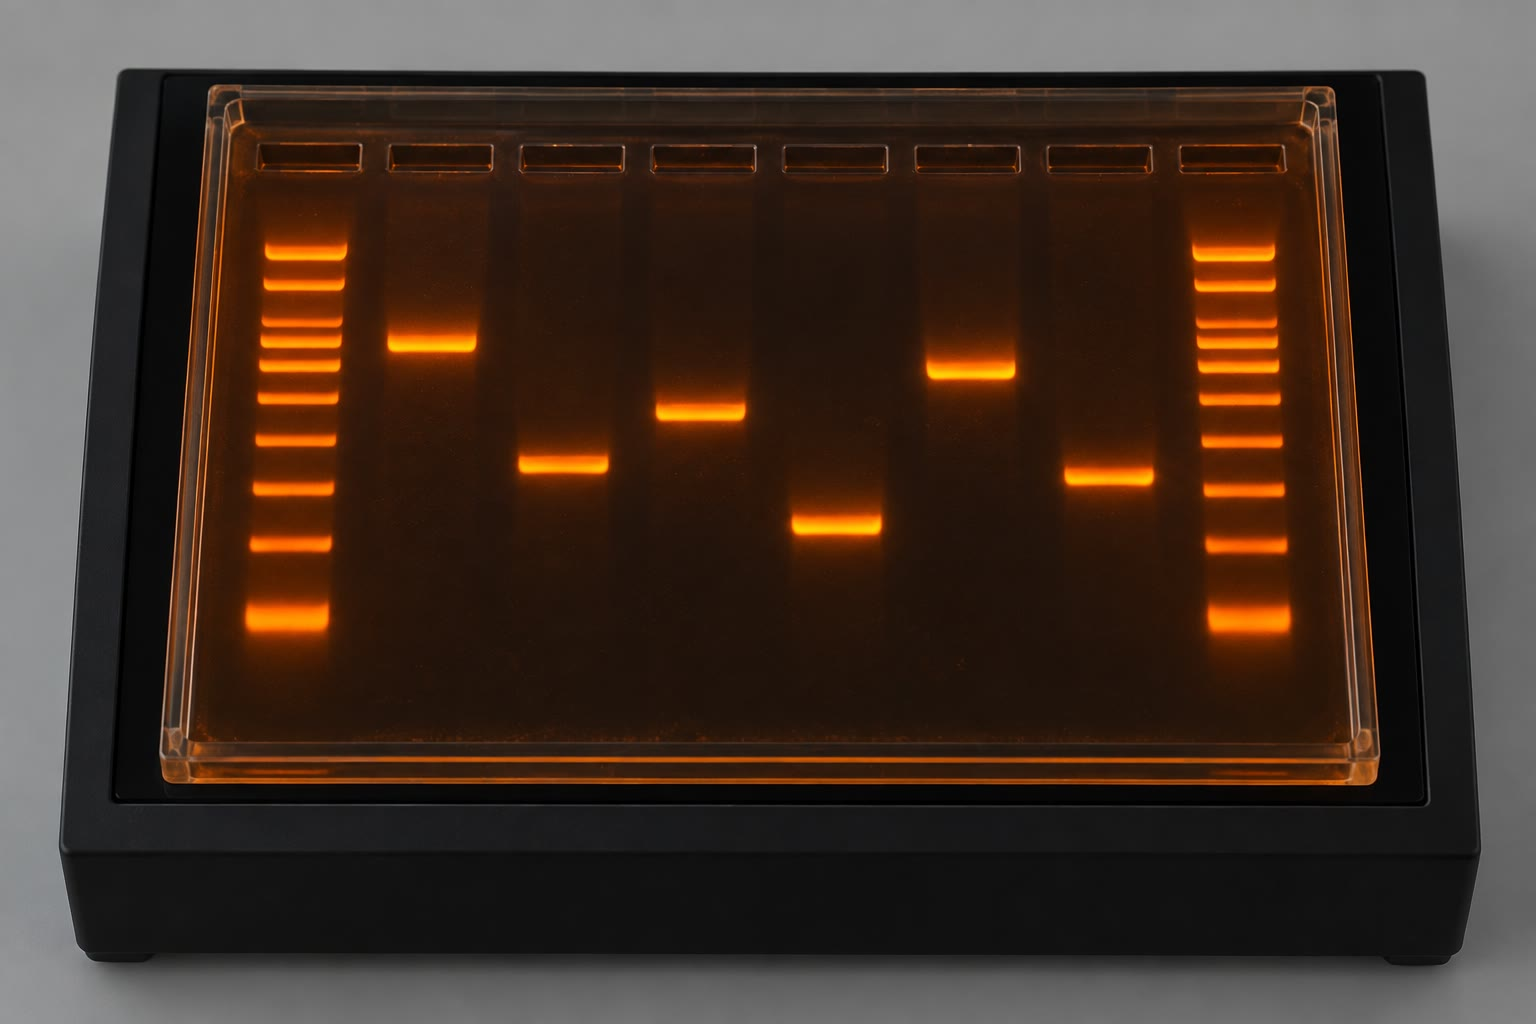
\includegraphics[width=0.56\linewidth]{images/book5/ai/b5-06-agarose-gel.jpg}

{\small An agarose gel under ultraviolet light: DNA fragments migrate
toward the anode at a speed that falls with their length, so each band
is a population of molecules of one size, compared with the ladder of
known sizes in the outer lanes.}
\end{omfigure}

\begin{definition}[The polymerase chain reaction]\label{def:b3:genetic-engineering:pcr}
\index{polymerase chain reaction}\index{primer}\index{quantitative PCR}
The \emph{polymerase chain reaction} (PCR) amplifies a chosen stretch
of DNA between two \emph{primers} --- synthetic oligonucleotides of
about twenty bases complementary to the two strands at the ends of the
target --- through cycles of three temperatures: \qty{95}{\celsius} to
separate the strands, \qtyrange{50}{65}{\celsius} for the primers to
anneal, \qty{72}{\celsius} for a heat-stable polymerase (Taq, from the
hot-spring bacterium \emph{Thermus aquaticus}) to extend them. Each
cycle doubles the number of copies of the segment between the primers,
so thirty cycles turn a single molecule into a billion. \emph{Reverse
transcription PCR} first copies RNA into DNA and so measures
transcripts or RNA viruses; \emph{quantitative PCR} (qPCR) follows the
amplification in real time with a fluorescent dye and reads the
starting quantity from the cycle at which the signal crosses a
threshold.
\end{definition}

\begin{theorem}[The arithmetic of amplification]\label{thm:b3:genetic-engineering:pcr}
\index{threshold cycle}
With efficiency $E$ per cycle ($E = 1$ for perfect doubling), $N_{0}$
starting copies become
\[
N_{n} = N_{0}\,(1 + E)^{n}
\]
after $n$ cycles. If the fluorescence crosses a fixed threshold when
the copy number reaches $N_{T}$, the \emph{\omterm{thm:b3:genetic-engineering:pcr}{threshold cycle}} is
\[
C_{T} = \frac{\log N_{T} - \log N_{0}}{\log(1 + E)},
\]
a straight line in $\log N_{0}$ with slope $-1/\log(1+E)$: for $E = 1$,
each tenfold increase in the starting quantity lowers $C_{T}$ by
$\log_{2} 10 = 3.32$ cycles, and two samples with \omterm{thm:b3:genetic-engineering:pcr}{threshold cycles}
differing by $\Delta C_{T}$ differ in starting copies by the factor
$(1 + E)^{\Delta C_{T}}$.
\end{theorem}
\begin{proof}
Each cycle multiplies the copy number by $1 + E$, so $N_{n}$ is a
geometric sequence. Setting $N_{n} = N_{T}$ and solving for $n$ gives
$C_{T}$; the slope is the coefficient of $\log N_{0}$. For two samples,
$C_{T,1} - C_{T,2} = (\log N_{0,2} - \log N_{0,1})/\log(1+E)$, whence
$N_{0,2}/N_{0,1} = (1+E)^{\Delta C_{T}}$.
\end{proof}

\begin{example}[Reading a qPCR plate]\label{ex:b3:genetic-engineering:qpcr}
A viral RNA test crosses the threshold at cycle $22$ for one patient
and cycle $32$ for another; with $E \approx 1$ the first carries $2^{10}
\approx 1000$ times more virus. A sample of ten copies crosses at about
cycle $37$ when the threshold is $10^{12}$ copies ($\log_{2} 10^{11} =
36.5$); a run of $40$ cycles therefore detects a few molecules, and a
single contaminating molecule of a previous amplicon does too, which is
why laboratories separate the rooms where PCR is set up from those
where products are handled.
\end{example}

\begin{omfigure}
\begin{tikzpicture}
\begin{axis}[
  width=0.7\linewidth, height=5.6cm,
  axis x line=bottom, axis y line=left,
  xmin=0, xmax=40, ymin=1, ymax=1e14, ymode=log,
  xlabel={cycle}, ylabel={copies},
  xlabel style={font=\small, at={(axis description cs:0.5,-0.12)}, anchor=north},
  ylabel style={font=\small},
  tick label style={font=\small}, xtick={0,10,20,30,40},
  clip=false,
]
\addplot[very thick, omDef, domain=0:40, samples=41] {1e7*2^x/(1+2^x/1e5)};
\addplot[very thick, omThm, domain=0:40, samples=41] {1e4*2^x/(1+2^x/1e8)};
\addplot[very thick, omMeth!70!black, domain=0:40, samples=41] {10*2^x/(1+2^x/1e11)};
\addplot[dashed, gray, domain=0:40, samples=2] {1e12};
\node[font=\scriptsize, gray, anchor=south west] at (axis cs:0.5,1.3e12) {threshold $N_{T}$};
\draw[gray] (axis cs:16.6,1) -- (axis cs:16.6,1e12); \draw[gray] (axis cs:26.6,1) -- (axis cs:26.6,1e12); \draw[gray] (axis cs:36.5,1) -- (axis cs:36.5,1e12);
\node[font=\scriptsize, anchor=south] at (axis cs:16.6,3e12) {$C_{T} = 16.6$}; \node[font=\scriptsize, anchor=south] at (axis cs:26.6,3e12) {$26.6$}; \node[font=\scriptsize, anchor=south] at (axis cs:36.5,3e12) {$36.5$};
\end{axis}
\end{tikzpicture}

{\small Amplification curves for $N_{0} = 10^{7}$ (blue), $10^{4}$ (red)
and $10$ copies (green), $E = 1$, with the plateau that reagents impose. A thousandfold difference in
$N_{0}$ shifts the \omterm{thm:b3:genetic-engineering:pcr}{threshold cycle} by $10$; the plateaus are all alike,
which is why the end product tells nothing about the start.}
\end{omfigure}

\section{Making proteins}

\begin{definition}[Expression systems]\label{def:b3:genetic-engineering:expression}
\index{expression vector}\index{recombinant protein}\index{monoclonal antibody}
An \emph{expression \omterm{def:b3:genetic-engineering:tools}{vector}} places the cloned coding sequence under a
strong, controllable promoter of the host (the \emph{lac} or T7
promoter in \emph{E.~coli}, induced by a sugar analogue), with a
ribosome-binding site, a terminator, and often a \emph{tag} --- six
histidines, a small protein --- fused to the product for purification
on a column. Bacteria make grams per litre of a simple protein
(insulin, growth hormone, enzymes) but cannot glycosylate or fold
complex mammalian proteins; yeast adds sugars of its own kind; insect
and mammalian cells (Chinese hamster ovary cells are the industry's
standard) make antibodies and clotting factors folded and glycosylated
as in a human. A \emph{monoclonal antibody} is made by a
\emph{hybridoma} --- an antibody-producing B~cell fused to an immortal
myeloma cell (K\"ohler and Milstein, 1975) --- or, now, by cloning the
antibody genes into a mammalian expression line, where the mouse
framework can be replaced by human sequence to avoid immune rejection
(\cref{ch:b3:adaptive-immunity}).
\end{definition}

\begin{example}[Insulin]\label{ex:b3:genetic-engineering:insulin}
Human insulin is two chains, A (21 residues) and B (30), joined by
disulfide bonds, cut in the $\beta$ cell from a single proinsulin
precursor. The first process expressed the two chains separately in
\emph{E.~coli}, each fused to $\beta$-galactosidase, cleaved them off
chemically and joined them in vitro; later processes express proinsulin
and cleave it with the enzymes the pancreas uses. Since 1996 the
sequence itself has been altered: swapping or adding a residue or two
gives analogues that dissociate faster (for a meal) or precipitate at
the injection site and release over a day. A protein that took eight
tonnes of glands per kilogram is now made in a fermenter, identical to
the human one or better than it.
\end{example}

\section{Transgenic organisms}

\begin{definition}[Transgenesis and gene targeting]\label{def:b3:genetic-engineering:transgenic}
\index{transgenic organism}\index{microinjection}\index{knockout}\index{embryonic stem cell}\index{gene targeting}
A \emph{transgenic} organism carries a gene introduced into its germ
line, so that every cell has it and it is inherited. In mice the
classical route is \emph{microinjection} of the DNA into one pronucleus
of a fertilised egg (Gordon and Ruddle, 1980), which integrates at a
random site in a fraction of embryos; Palmiter and Brinster (1982) made
mice twice normal size by injecting the rat growth-hormone gene behind
a metallothionein promoter. \emph{Gene targeting} replaces or disrupts
a chosen gene instead: a construct with long arms homologous to the
target is introduced into \emph{embryonic stem cells}, the rare cells
in which \omterm{def:b3:dna-repair:dsb}{homologous recombination} has put it in the right place are
selected and injected into a blastocyst, and the chimaeric mouse that
results transmits the altered gene (Capecchi, Smithies and Evans,
1980s). A \emph{knockout} lacks the gene; a \emph{knock-in} carries a
modified version; a \emph{conditional} allele, flanked by loxP sites, is
deleted only where and when Cre is expressed
(\cref{ch:b3:dna-repair}). Some ten thousand mouse genes have been
knocked out, and for most the phenotype was the first indication of
what the gene does.
\end{definition}

\begin{omfigure}
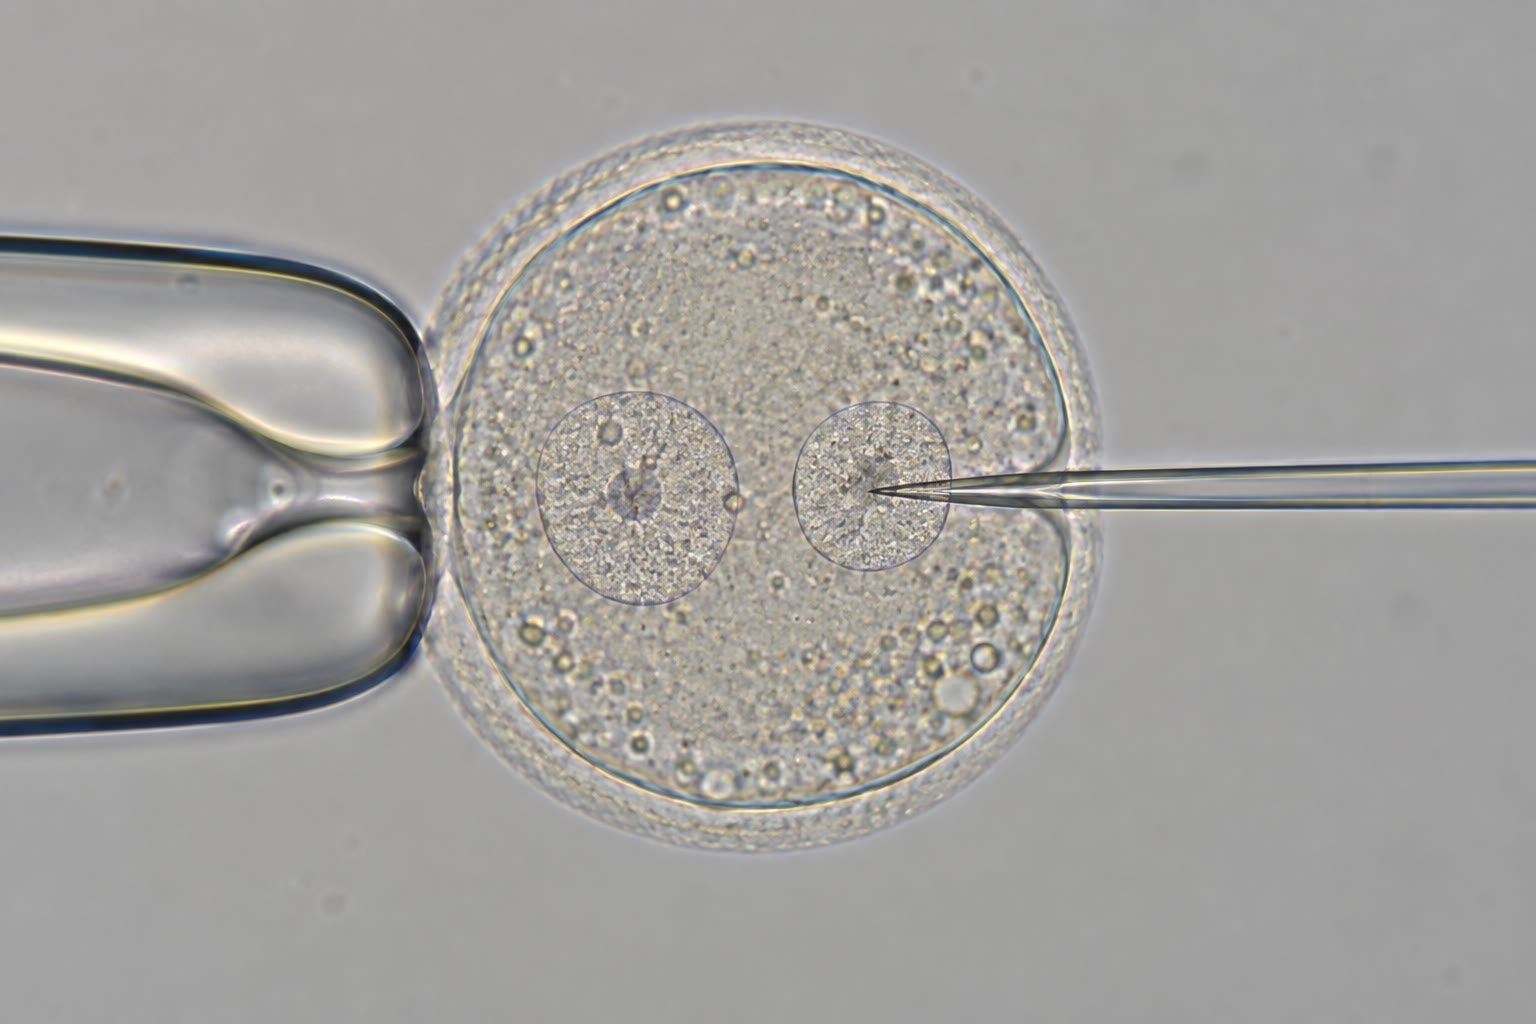
\includegraphics[width=0.46\linewidth]{images/book5/ai/b5-06-microinjection.jpg}\hspace{0.04\linewidth}
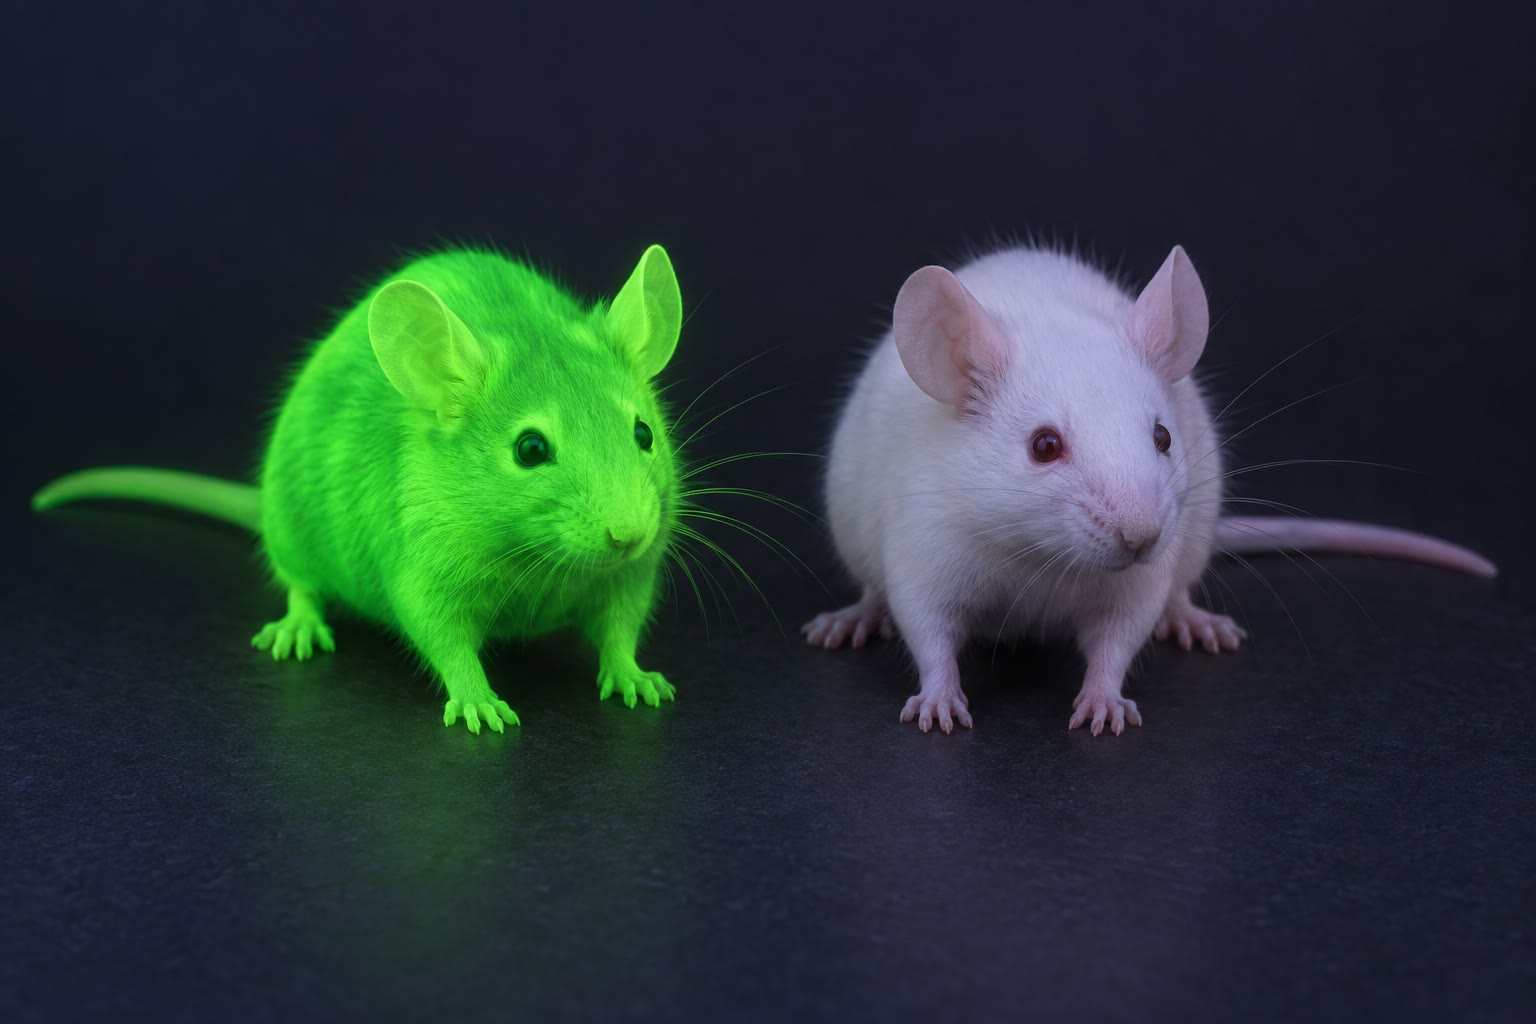
\includegraphics[width=0.46\linewidth]{images/book5/ai/b5-06-gfp-mouse.jpg}

{\small Left: a fertilised mouse egg held by suction while a glass
needle injects DNA into one pronucleus. Right: a \omterm{def:b3:genetic-engineering:transgenic}{transgenic} mouse
expressing the green fluorescent protein of a jellyfish in every cell,
beside an ordinary littermate, under ultraviolet light.}
\end{omfigure}

\begin{definition}[Transgenic plants]\label{def:b3:genetic-engineering:plants}
\index{Agrobacterium}\index{T-DNA}\index{genetically modified crop}
Plants are transformed by \emph{Agrobacterium tumefaciens}, a soil
bacterium that naturally inserts a segment of its tumour-inducing
\omterm{def:b3:genetic-engineering:tools}{plasmid}, the \emph{T-DNA}, into the genome of a wounded plant to make
it grow a gall and feed the bacterium. Replacing the T-DNA's own genes
with any gene of choice, between the border sequences the bacterium
recognises, turns the pathogen into a \omterm{def:b3:genetic-engineering:tools}{vector}; the transformed cells
are selected and regenerated into whole plants, which every plant
cell can do. Species the bacterium does not infect (the cereals, for
long) are transformed by shooting DNA-coated gold particles into
tissue. \emph{Genetically modified crops} grown at scale carry a
bacterial toxin gene (\emph{Bt}) against insect larvae, or a bacterial
enzyme conferring tolerance to a herbicide, or both; \emph{Golden Rice}
carries two genes of the carotenoid pathway (a plant phytoene synthase
and a bacterial desaturase) so that its endosperm makes
$\beta$-carotene, the precursor of vitamin~A, whose deficiency blinds
and kills several hundred thousand children a year.
\end{definition}

\begin{omfigure}
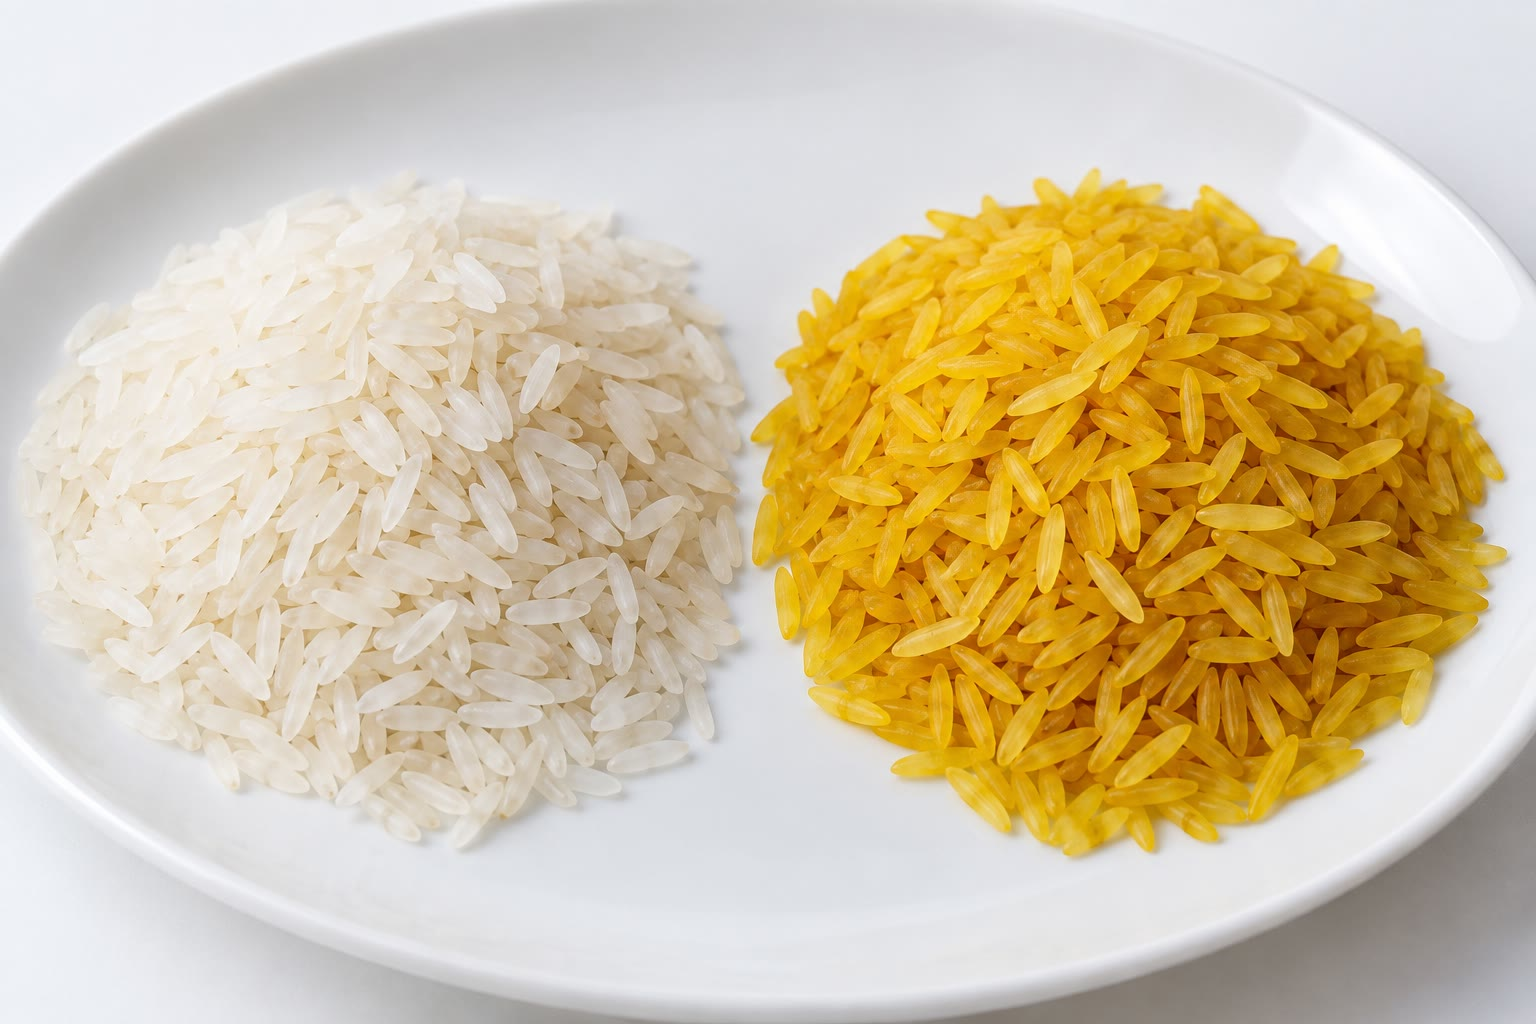
\includegraphics[width=0.46\linewidth]{images/book5/ai/b5-06-golden-rice.jpg}\hspace{0.04\linewidth}
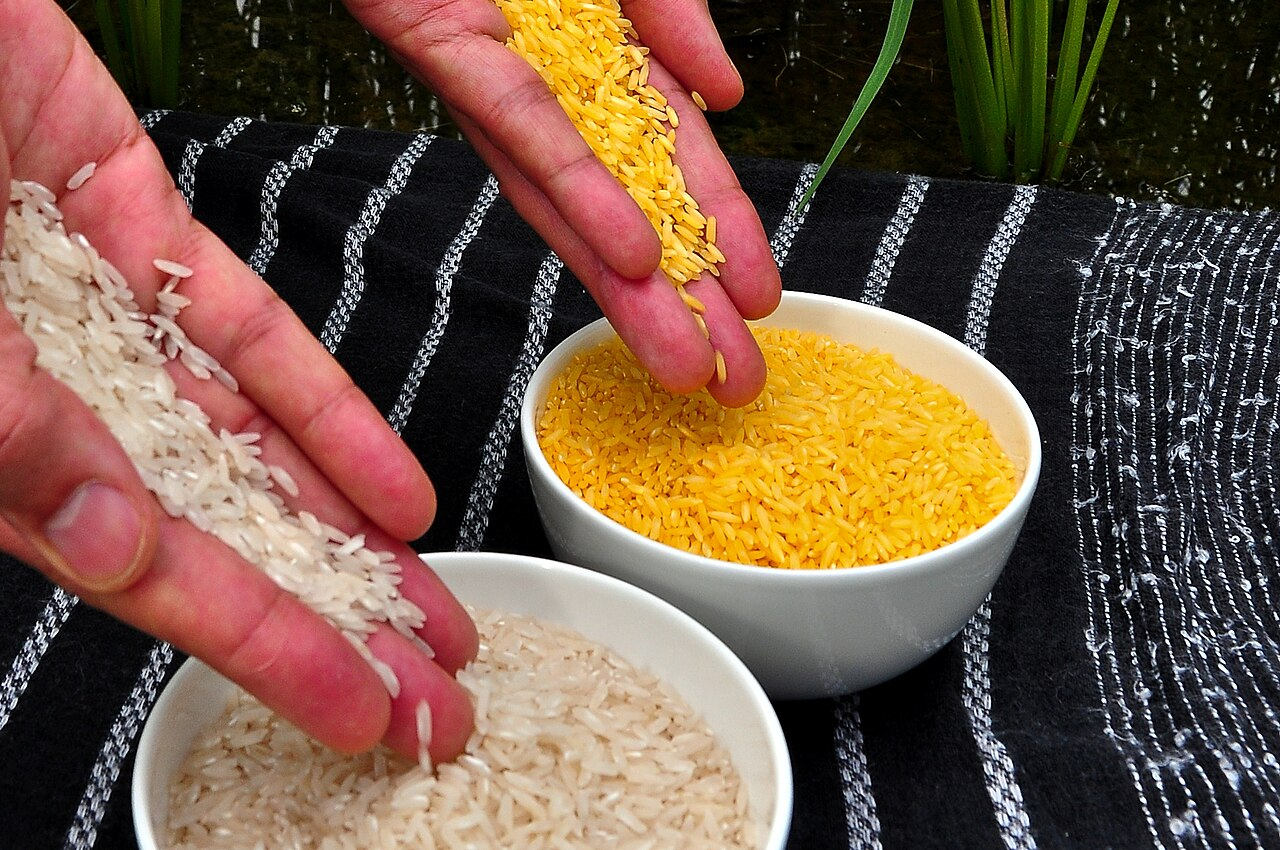
\includegraphics[width=0.46\linewidth]{images/book5/golden-rice-irri.jpg}

{\small Ordinary and Golden Rice. The yellow grain makes
$\beta$-carotene in its endosperm from two added genes of the
carotenoid pathway. Right: the two rices compared at the
International Rice Research Institute (IRRI, CC~BY~2.0).}
\end{omfigure}

\begin{remark}[The debate]\label{rem:b3:genetic-engineering:gmo}
Thirty years of cultivation on hundreds of millions of hectares, and
every systematic review by scientific academies, have found no health
effect of approved \omterm{def:b3:genetic-engineering:transgenic}{transgenic} crops that differs from their
conventional counterparts; the transgene is one more gene among forty
thousand, and the protein it makes is tested as any food additive is.
The real questions are ecological and economic: the spread of
resistance in pests and weeds under uniform selection, gene flow into
wild relatives, the concentration of the seed market, and who
benefits. They are the questions that any powerful agricultural
technology raises, and the answers depend on the trait and the
setting, not on the method by which the gene was moved.
\end{remark}

\section{Editing genomes}

\begin{definition}[CRISPR--Cas9]\label{def:b3:genetic-engineering:crispr}
\index{CRISPR}\index{Cas9}\index{guide RNA}\index{PAM}\index{genome editing}
Bacteria store fragments of the genomes of phages that have infected
their ancestors in an array of repeats (\emph{CRISPR}), transcribe them
into short guide RNAs, and use them to direct a nuclease to cut any
matching DNA that enters the cell: an adaptive immune system with a
genetic memory. In \emph{Streptococcus pyogenes} the nuclease is the
single protein \emph{Cas9}, which binds a guide RNA and a second small
RNA, searches DNA for a three-base \emph{protospacer-adjacent \omterm{def:b3:bioinformatics:motif}{motif}}
(PAM, 5$'$-NGG), unwinds the adjacent DNA, and, if the twenty bases
next to the PAM pair with the guide, cuts both strands three bases from
the PAM. Jinek, Charpentier, Doudna and colleagues (2012) fused the two
RNAs into one \emph{single-guide RNA} and showed that Cas9 with a guide
of any chosen sequence cuts DNA at that sequence in a test tube; within
a year the pair had been shown to work in human, mouse, zebrafish,
plant and yeast cells. \emph{Genome editing} is what the cell does
with the cut: end joining leaves a small insertion or deletion that
disrupts the gene (a \omterm{def:b3:genetic-engineering:transgenic}{knockout} in one step, in any organism, in weeks),
and \omterm{def:b3:dna-repair:dsb}{homologous recombination} with a supplied template writes in a
chosen sequence.
\end{definition}

\begin{omfigure}
\begin{tikzpicture}[every node/.style={font=\scriptsize}, >=stealth]
  % Cas9 outline (drawn first so labels stay on top)
  \draw[thick, omExo, fill=omExo!15] (5.9,1.1) ellipse (2.6 and 1.6);
  \node[omExo!60!black] at (7.7,2.3) {Cas9};
  % target DNA
  \draw[very thick, omDef] (0,0.3) -- (11,0.3); \draw[very thick, omDef] (0,-0.1) -- (11,-0.1);
  % PAM
  \fill[omProp!60] (7.2,-0.2) rectangle (7.9,0.4); \node[below] at (7.55,-0.25) {PAM (NGG)};
  % protospacer
  \draw[omThm, very thick] (4.2,0.5) -- (7.15,0.5); \node[above] at (5.7,0.55) {20-base target, paired with the guide};
  % guide RNA
  \draw[very thick, omMeth!70!black] (4.2,0.3) .. controls (4.2,1.6) and (5.0,1.9) .. (5.4,1.9) -- (6.6,1.9) .. controls (7.0,1.9) and (7.2,2.5) .. (6.8,2.8) .. controls (6.3,3.1) and (5.8,2.7) .. (6.1,2.4);
  \node[left, omMeth!70!black, align=right] at (3.2,2.2) {single-guide RNA:\\20 bases of choice\\+ Cas9-binding hairpin};
  % cut
  \draw[omThm, very thick, ->] (6.25,-0.7) -- (6.25,0.35); \node[omThm, below] at (6.25,-0.7) {double-strand break, 3 bases from the PAM};
  % outcomes
  \draw[->, thick] (2.0,-1.3) -- (2.0,-1.9); \node[below, align=center] at (2.0,-1.9) {end joining:\\small insertion or deletion\\$\Rightarrow$ frameshift, knockout};
  \draw[->, thick] (10.0,-1.3) -- (10.0,-1.9); \node[below, align=center] at (10.0,-1.9) {recombination with a\\supplied template\\$\Rightarrow$ precise change};
\end{tikzpicture}

{\small \omterm{def:b3:genetic-engineering:crispr}{Cas9} and its guide. The protein binds a \omterm{def:b3:genetic-engineering:crispr}{PAM}, unwinds the DNA
next to it, and cuts if the twenty bases pair with the \omterm{def:b3:genetic-engineering:crispr}{guide RNA}. The
break is repaired either by end joining, which disrupts the gene, or by
recombination with a template, which rewrites it.}
\end{omfigure}

\begin{proposition}[Editing without a break]\label{prop:b3:genetic-engineering:editors}
\index{base editor}\index{prime editor}\index{off-target}
Cutting both strands is the crudest edit: the outcome of end joining is
random, and a break elsewhere --- an \emph{off-target} site differing
from the guide at a few positions, which \omterm{def:b3:genetic-engineering:crispr}{Cas9} tolerates --- is a
mutation nobody asked for. A \omterm{def:b3:genetic-engineering:crispr}{Cas9} with one nuclease domain inactivated
nicks a single strand; with both inactivated it merely binds, and can
carry other enzymes to a sequence. \emph{\omterm{prop:b3:genetic-engineering:editors}{Base editors}} fuse a
nicking \omterm{def:b3:genetic-engineering:crispr}{Cas9} to a deaminase that converts C to U (read as T) or A to I
(read as G) in the unwound strand, changing one base without a break
and without a template; \emph{\omterm{prop:b3:genetic-engineering:editors}{prime editors}} carry a reverse
transcriptase and a guide extended with the desired sequence, and copy
that sequence into the nicked strand, allowing any substitution and
small insertions or deletions. Off-target activity is reduced by
engineered high-fidelity \omterm{def:b3:genetic-engineering:crispr}{Cas9} variants, by delivering the enzyme
briefly as protein rather than as a gene, and by choosing guides whose
nearest genomic relatives differ at several positions; it is measured
by sequencing the sites predicted, and by unbiased methods that catch
every break in the genome.
\end{proposition}

\begin{example}[A cure]\label{ex:b3:genetic-engineering:sickle}
Sickle-cell disease is a single base change in $\beta$-globin. Fetal
haemoglobin, made from $\gamma$-globin, would substitute, but the
$\gamma$ genes are switched off after birth by the repressor BCL11A.
The first approved \omterm{def:b3:genetic-engineering:crispr}{CRISPR} therapy (2023) takes the patient's own blood
stem cells, cuts the erythroid enhancer of \emph{BCL11A} with \omterm{def:b3:genetic-engineering:crispr}{Cas9} so
that end joining disables it in most cells, and returns the cells after
the patient's marrow has been cleared: the red cells they make are rich
in fetal haemoglobin, do not sickle, and the crises stop. The edit is
somatic --- the germ line is untouched and the change is not inherited
--- and it uses the ``crude'' outcome, disruption, where disruption is
what is wanted.
\end{example}

\begin{theorem}[Super-Mendelian spread of a gene drive]\label{thm:b3:genetic-engineering:drive}
\index{gene drive}
A \emph{\omterm{thm:b3:genetic-engineering:drive}{gene drive}} is a construct encoding \omterm{def:b3:genetic-engineering:crispr}{Cas9} and a guide that cuts
the wild-type allele at its own locus in a heterozygote; repair by
recombination copies the drive into the cut chromosome, so that a
fraction $c$ of the heterozygote's gametes carry the drive instead of
the Mendelian half. If the drive has frequency $p$ in a large,
randomly mating population and no fitness cost, its frequency in the
next generation is
\[
p' = p + c\,p\,(1 - p),
\]
so that it spreads from rarity at a rate proportional to $c$, and
reaches half the population in about $\ln(1/p_{0})/\ln(1 + c)$
generations from an initial frequency $p_{0}$.
\end{theorem}
\begin{proof}
Random mating gives homozygotes for the drive at frequency $p^{2}$,
heterozygotes at $2p(1-p)$, wild-type homozygotes at $(1-p)^{2}$. The
homozygotes transmit the drive to all their gametes, the heterozygotes
to a fraction $(1 + c)/2$ (half by Mendel, plus $c$ times the wild-type
half converted), the wild-type to none. Hence $p' = p^{2} + 2p(1-p)(1+c)/2
= p^{2} + p(1-p) + c\,p(1-p) = p + c\,p(1-p)$. For small $p$ this is
$p' \approx (1+c)p$, geometric growth with ratio $1 + c$, which reaches
$1/2$ from $p_{0}$ after about $\ln(1/2p_{0})/\ln(1+c)$ generations; the
logistic term slows it only near the end.
\end{proof}

\begin{omfigure}
\begin{tikzpicture}
\begin{axis}[
  width=0.7\linewidth, height=5.6cm,
  axis x line=bottom, axis y line=left,
  xmin=0, xmax=20, ymin=0, ymax=1.05,
  xlabel={generation}, ylabel={drive frequency $p$},
  xlabel style={font=\small, at={(axis description cs:0.5,-0.12)}, anchor=north},
  ylabel style={font=\small},
  tick label style={font=\small}, xtick={0,5,10,15,20}, ytick={0,0.5,1},
  clip=false,
]
\addplot[very thick, omThm, mark=*, mark size=1.2pt] coordinates {(0,0.01) (1,0.0189) (2,0.0356) (3,0.0665) (4,0.1224) (5,0.2191) (6,0.3731) (7,0.5836) (8,0.8023) (9,0.9451) (10,0.9918) (11,0.9991) (12,1.0) (13,1.0) (14,1.0) (15,1.0) (16,1.0) (17,1.0) (18,1.0) (19,1.0) (20,1.0)};
\addplot[very thick, omDef, mark=*, mark size=1.2pt] coordinates {(0,0.01) (1,0.015) (2,0.0223) (3,0.0332) (4,0.0493) (5,0.0727) (6,0.1064) (7,0.154) (8,0.2191) (9,0.3047) (10,0.4106) (11,0.5316) (12,0.6561) (13,0.769) (14,0.8578) (15,0.9188) (16,0.9561) (17,0.9771) (18,0.9883) (19,0.9941) (20,0.997)};
\addplot[very thick, gray, dashed, domain=0:20, samples=2] {0.01};
\node[font=\scriptsize, omThm, anchor=south east] at (axis cs:6.5,0.62) {$c = 0.9$};
\node[font=\scriptsize, omDef, anchor=north west] at (axis cs:12.5,0.62) {$c = 0.5$};
\node[font=\scriptsize, gray, anchor=south west] at (axis cs:12,0.02) {Mendelian, $c = 0$: stays at $p_{0}$};
\end{axis}
\end{tikzpicture}

{\small A \omterm{thm:b3:genetic-engineering:drive}{gene drive} released at one percent, with conversion
efficiency $0.9$ or $0.5$ and no fitness cost. A Mendelian allele with
no advantage would stay at one percent; the drive takes over in ten or
twenty generations.}
\end{omfigure}

\begin{remark}[What may be edited]\label{rem:b3:genetic-engineering:ethics}
Editing the somatic cells of a consenting patient is medicine, judged
like any treatment by its risks and benefits. Editing the germ line ---
an embryo, whose every descendant would carry the change --- is
different in kind: the person affected cannot consent, the change is
inherited, and the technique's off-target and mosaic outcomes are not
yet controlled; after a Chinese scientist announced in 2018 that he
had done it in twins, the scientific academies of most countries called
for a moratorium and several states made it a crime. A \omterm{thm:b3:genetic-engineering:drive}{gene drive}
released into a wild population is a decision taken for everyone
downstream, which is why the field's own proposals for eliminating
malaria mosquitoes couple the drives to fail-safes --- reversal drives,
self-limiting designs --- and to public consent in the countries
concerned.
\end{remark}

\section{Exercises}

\begin{exercise}[$\star$]\label{exo:b3:genetic-engineering:1}
List the three components a cloning \omterm{def:b3:genetic-engineering:tools}{plasmid} must have and explain the
purpose of each.
\end{exercise}

\begin{exercise}[$\star$]\label{exo:b3:genetic-engineering:2}
EcoRI recognises GAATTC. How often does the site occur, on average, in
random DNA, and how many fragments does it make of the \qty{4.6}{Mb}
\emph{E.~coli} genome? Why is the real number somewhat different?
\end{exercise}

\begin{exercise}[$\star$]\label{exo:b3:genetic-engineering:3}
State the three temperature steps of a PCR cycle and what happens at
each. Why must the polymerase be heat-stable?
\end{exercise}

\begin{exercise}[$\star$]\label{exo:b3:genetic-engineering:4}
What does \omterm{def:b3:genetic-engineering:crispr}{Cas9} need in order to cut a given sequence, and what two
outcomes can follow the cut?
\end{exercise}

\begin{exercise}[$\star\star$]\label{exo:b3:genetic-engineering:5}
A PCR runs $35$ cycles at efficiency $E = 0.9$ from $50$ copies. How many
copies result? A qPCR of two samples gives $C_{T} = 18.2$ and $25.5$;
with $E = 0.95$, what is the ratio of their starting quantities?
\end{exercise}

\begin{exercise}[$\star\star$]\label{exo:b3:genetic-engineering:6}
Why is a cDNA library, and not a genomic library, used to express a
human protein in bacteria? Name two other obstacles to making a human
protein in \emph{E.~coli} and say how each is overcome.
\end{exercise}

\begin{exercise}[$\star\star$]\label{exo:b3:genetic-engineering:7}
A \omterm{def:b3:genetic-engineering:transgenic}{knockout} mouse is made by \omterm{def:b3:genetic-engineering:transgenic}{gene targeting} in \omterm{def:b3:genetic-engineering:transgenic}{embryonic stem cells}.
Explain why the first mouse born is a chimaera, why one must breed it,
and what fraction of the grandchildren of a chimaera whose germ line is
half targeted are homozygous \omterm{def:b3:genetic-engineering:transgenic}{knockouts} if heterozygous grandparents are
intercrossed.
\end{exercise}

\begin{exercise}[$\star\star$]\label{exo:b3:genetic-engineering:8}
A \omterm{def:b3:genetic-engineering:crispr}{guide RNA} of 20 bases with an NGG \omterm{def:b3:genetic-engineering:crispr}{PAM} is chosen. How many sites in a
$3.2\times 10^{9}$ bp genome (both strands) match the guide exactly by
chance? How many match with up to two mismatches, if \omterm{def:b3:genetic-engineering:crispr}{Cas9} tolerates
them? (Count sequences within two mismatches as $1 + 3\binom{20}{1} +
9\binom{20}{2}$.)
\end{exercise}

\begin{exercise}[$\star\star$]\label{exo:b3:genetic-engineering:9}
Using \cref{thm:b3:genetic-engineering:drive}, compute the frequency of
a drive with $c = 0.8$ after three generations from $p_{0} = 0.05$, and
estimate the number of generations to reach $0.5$.
\end{exercise}

\begin{exercise}[$\star\star\star$]\label{exo:b3:genetic-engineering:10}
The sickle-cell therapy disrupts an enhancer rather than correcting the
$\beta$-globin mutation. Give two reasons why disruption by end joining
was chosen over correction by \omterm{def:b3:dna-repair:dsb}{homologous recombination} in blood stem
cells, and one drawback.
\end{exercise}

\begin{exercise}[$\star\star\star$]\label{exo:b3:genetic-engineering:11}
A \omterm{thm:b3:genetic-engineering:drive}{gene drive} against a mosquito carries a fitness cost $s$ in
homozygotes. Modify the recursion to include selection against drive
homozygotes and find the condition on $c$ and $s$ for the drive to
spread from rarity. Then explain why resistance alleles --- end-joining
products at the target that the guide no longer recognises --- are the
principal obstacle in practice.
\end{exercise}

\begin{exercise}[$\star\star\star$]\label{exo:b3:genetic-engineering:12}
Argue, with the mechanisms of this chapter and of
\cref{ch:b3:dna-repair}, why germline editing of a human embryo cannot
at present guarantee the intended outcome in every cell, and what
evidence would be needed before a rational person could consider it
safe.
\end{exercise}

\section{Problem: From a Gene to a Drug and a Crop}

\begin{problem}[{Weekend problem --- a gene cloned with the arithmetic
of restriction sites and transformation, a virus counted by qPCR, a
hormone produced by the tonne in a fermenter, a genome edited with its
off-targets counted, and a gene drive timed, ending on the copies of a
virus in a sample, the annual fermenter volume for the world's insulin
and the number of generations a drive needs}]
\label{pb:b3:genetic-engineering:1}
Data: a \qty{1.5}{kb} gene; a six-base restriction site; a \omterm{def:b3:genetic-engineering:tools}{plasmid} of
\qty{4}{kb}; transformation efficiency $2\times 10^{7}$ colonies per
microgram of \omterm{def:b3:genetic-engineering:tools}{plasmid}; ligation gives \qty{10}{\%} of \omterm{def:b3:genetic-engineering:tools}{plasmids} an
insert. qPCR efficiency $E = 1$, threshold $N_{T} = 10^{12}$. Insulin:
\qty{5.8}{kDa}, a patient uses $40$ units a day, one unit being
\qty{35}{\micro g}; $10^{7}$ patients; a fermenter yields
\qty{2}{g/L} of product per batch, ten batches a year. Genome $3.2\times
10^{9}$ bp. Drive conversion $c = 0.9$, released at $p_{0} = 0.001$.

\medskip
\noindent\textbf{Part I --- Cloning.}
\begin{enumerate}
  \item How often does a given six-base site occur in random DNA? What
        is the probability that the \qty{1.5}{kb} gene contains no
        such site, so that the enzyme can be used to clone it whole?
  \item If it does contain a site, how would you clone it anyway?
        (Two methods.)
  \item \qty{100}{ng} of ligated \omterm{def:b3:genetic-engineering:tools}{plasmid} is transformed. How many
        colonies, and how many carry the insert?
  \item Blue--white screening is used. What fraction of colonies is
        white, and how many white colonies must be picked to have a
        \qty{99}{\%} chance that at least one carries the gene in the
        right orientation (half of the inserts)?
  \item The recombinant \omterm{def:b3:genetic-engineering:tools}{plasmid} is \qty{5.5}{kb}. A cell holds $50$
        copies and divides every \qty{30}{min}. After overnight growth
        (\qty{16}{h}) from one cell, how many \omterm{def:b3:genetic-engineering:tools}{plasmid} molecules, and
        what mass of \omterm{def:b3:genetic-engineering:tools}{plasmid} DNA (\qty{650}{Da} per base pair)?
  \item Why does the \omterm{def:b3:genetic-engineering:tools}{plasmid} need a bacterial origin but the inserted
        human gene need no bacterial promoter for cloning, whereas it
        does for expression?
\end{enumerate}

\medskip
\noindent\textbf{Part II --- Counting a virus.}
\begin{enumerate}[resume]
  \item A patient's sample crosses the threshold at $C_{T} = 28$. How
        many copies were in the reaction? Another at $C_{T} = 35$?
  \item Sensitivity: how many cycles are needed to bring a single copy
        to the threshold?
  \item The test's cut-off is set at $C_{T} = 38$. What number of
        copies does that correspond to, and why not use $45$ cycles?
  \item A contaminating molecule of a previous run's product enters a
        negative sample. At what cycle does it cross the threshold?
        What laboratory practice prevents this?
  \item Reverse transcription converts \qty{40}{\%} of viral RNA to
        DNA. Correct the count of question 7 for the first sample.
  \item Two samples differ by $\Delta C_{T} = 3.3$ with $E = 1$, but
        the efficiency is actually $0.9$. What fold difference does the
        analyst report, and what is the true one?
\end{enumerate}

\medskip
\noindent\textbf{Part III --- Insulin by the tonne.}
\begin{enumerate}[resume]
  \item Compute the daily insulin mass per patient and the annual
        world requirement for $10^{7}$ patients, in kilograms.
  \item How many moles of insulin is that, and how many molecules?
  \item What fermenter volume, run ten batches a year, produces it?
        Compare with a swimming pool of \qty{2500}{m^3}.
  \item Extraction from glands gave \qty{1}{kg} of insulin per
        \qty{8000}{kg} of pancreas; a pig pancreas weighs
        \qty{100}{g}. How many pigs a year would the world need?
  \item Why is the recombinant hormone preferred even where animal
        insulin is cheap? Give two reasons.
  \item Insulin analogues differ from the human sequence by one or two
        residues. Explain why an analogue is still a drug that acts on
        the human receptor, and why a change of one residue can alter
        its dissociation time.
\end{enumerate}

\medskip
\noindent\textbf{Part IV --- Editing and driving.}
\begin{enumerate}[resume]
  \item How many exact matches of a 20-base guide plus NGG does the
        genome contain by chance (both strands: $6.4\times 10^{9}$
        positions)?
  \item If \omterm{def:b3:genetic-engineering:crispr}{Cas9} tolerates up to three mismatches, how many sequences
        are within three mismatches of the guide, and how many chance
        off-target sites result?
  \item The edited blood stem cells are $10^{7}$; \qty{80}{\%} carry
        the intended disruption. How many cells carry an off-target
        break at a given site if it is cut in one cell in $10^{4}$,
        and why is a break in a tumour-suppressor gene in a single
        stem cell a concern?
  \item Compute the drive's frequency after $1, 2, 3$ generations from
        $p_{0} = 0.001$, and estimate the generations to $0.5$.
  \item A mosquito has ten generations a year. How many years to take
        over? How does a fitness cost of \qty{20}{\%} in homozygotes
        change the picture qualitatively?
  \item A resistance allele arises when end joining, not recombination,
        repairs the cut, with probability $1 - c = 0.1$ per conversion
        attempt. Estimate the number of resistance alleles created in
        a population of $10^{6}$ heterozygotes in one generation, and
        explain what happens to the drive if they are fit.
  \item Summarise: the copies in the first sample (question~7), the
        world's annual insulin fermenter volume (question~15), and the
        generations for the drive to reach half the population
        (question~22).
\end{enumerate}
\end{problem}
